% Chapter 1

\chapter{Grundlagen} % Main chapter title

\label{Chapter2} % For referencing the chapter elsewhere, use \ref{Chapter1} 

%----------------------------------------------------------------------------------------

% Define some commands to keep the formatting separated from the content 


%----------------------------------------------------------------------------------------



Das folgende Kapitel dient dazu die in der Einleitung genannten Begriffe und Prinzipien genauer zu erläutern. Wir wollen also zunächst BPMN und die Bestandteile der Modellierungssprache genauer betrachten. Hierzu werden wir jedes Element einzeln betrachten dadurch stück für Stück ein passendes Beispiel erstellen. Dieses Beispiel wird auch im Rest der Arbeit Relevanz finden. 
Im Anschluss wird dann die verwendete Prozessalgebra genauer betrachtet. Auch hier wollen wir jeden Bestandteil des Modells im Detail erläutern.


\section{BPMN}
Wie in der Einleitung bereits erwähnt, dient BPMN der graphischen Darstellung von Business Prozessen. In BPMN werden diese Prozesse in einzelne Aktivitäten oder Aufgaben unterteilt und dann in der richtigen Reihenfolge aufgezeichnet. Es gibt unterschiedliche Möglichkeiten Verzweigungen, Abhängigkeiten und Ähnliches zu Modellieren doch zum größten Teil basiert alles auf der korrekten Aneinanderreihung dieser Aktivitäten.
\subsection{Erste Schritte - Events und Aktivitäten}

Im folgenden Abschnitt schauen wir uns also die von uns verwendete Teilmenge der Modellierungssprache BPMN an. Hierzu möchten wir zunächst einen einführenden Prozess als Beispiel betrachten. Für alle möglichen Homepages und Websites von unterschiedlichen Firmen und Anbietern können Konten erstellt werden. Diese dienen zur Wiedererkennung eines Kunden oder Mitarbeiters. In diesem Abschnitt wollen wir ein BPMN-Diagramm erstellen, welches den Registrierungsprozess auf einer solchen Website darstellen könnte. Wir werden die Modellierungssprache hierzu aufteilen und jeden Bestandteil der Sprache anhand des Beispiels einzeln erläutern so, dass wir am ende dieses Abschnittes ein erstes, vollständiges Diagramm vorfinden. 
Die von uns genutzte Teilmenge kann in einzelne Blöcke eingeteilt werden. Diese können in zwei Gruppen unterteilt werden. Die Basic Blocks und die Flow Blocks. Des Weiteren kann unterschieden werden zwischen „Leaf Blocks“ und „Nonleaf Blocks.“ Alle Nonleaf Blocks bestehen aus beliebig vielen Leaf Blocks. Es existieren genau zwei für uns relevante Leaf Blocks, welche wir hier zunächst erwähnen möchten, um deren Funktion genauer zu erläutern. Die unterschiedlichen Blöcke sind jeweils durch sogenannte „sequnce flows“ verbunden. Diese werden dargestellt durch eine durchgezogene Linie mit einem ausgefüllten Pfeil am Ende. Sie verdeutlichen den Fluss des Diagrammes. Jeder Block hat einen eingehenden und einen ausgehenden Flow. Um zu verdeutlichen in welchem Zustand der Prozess sich zu einem bestimmten Zeitpunkt befindet, verwenden wir sogenannte Token. Diese beinhalten keine Daten, sondern stellen nur dar, welcher Teil des Prozesses gerade aufgeführt wird. Beim Ausführen des Prozesses wird ein Token immer in Richtung der Sequence Flows weitergegeben. Bei dem „Task Block“ und dem „Event Block“ handelt es sich um die beiden relevanten leaf-Blocks. Beide Blöcke werden durch den Namen bereits gut erklärt. Der Task Block, welcher durch ein abgerundetes Rechteckt dargestellt wird, ist repräsentativ für eine beliebige Aufgabe. Diese Aufgaben benötigen in jedem Fall Zeit, um ausgeführt zu werden. Er kann durch einen Text in der Mitte des Rechtecks beliebig benannt werden. Diese Aufgaben können jede erdenkliche Form annehmen. Eine Mögliche Aufgabe ist in Abbildung 2.1 dargestellt. Es handelt sich um das Eingeben der Anmeldedaten. Es handelt sich hierbei um eine Aufgabe die Zeit beansprucht und vom Nutzer ausgeführt wird. Sie ist offensichtlich relevant für unser Beispiel. 

\begin{figure}
\centering
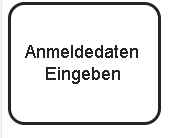
\includegraphics[height=2.5cm]{Figures/Beispiel1}
\decoRule
\caption[Einfache Task]{Einfache Task - Anmeldedaten eingeben}
\label{fig:Task}
\end{figure}

Bei dem zweiten Leaf Block handelt es sich nun um sogenannte Events. Events werden durch einen Kreis dargestellt. Anders als die Aufgaben passieren Events sofort. Es gibt unterschiedliche Typen, welche durch unterschiedliche Variationen eines Kreises dargestellt werden. Für uns relevant sind allerdings nur sogenannte „catching Events.“ Erreicht der Token ein solches Event, wird gewartet bis das erwartete Event auftritt und erst dann wird der Token weitergeschickt. Auch unter den catching Events gibt es drei grundsätzliche Unterscheidungen. Die einfachsten Variationen sind sogenannte Startevents, welche einen Prozess Starten und durch einen einfachen dünn gezeichneten Kreis dargestellt werden und die Endevents, welche den Prozess terminieren und durch einen einfachen dick gezeichneten Kreis dargestellt werden. 
Durch die uns nun bekannten Bausteine, ist es uns möglich einen ersten Prozess aufzubauen und in BPMN zu Modellieren. In Abbildung 2.2 sehen wir ein Beispiel für den ersten und einfachsten „nonleaf-Block.“ Den „Prozess-Block.“ Dieser besteht aus einem Start- und einem Endevent. Zwischen den beiden Events liegt mindestens ein Task-Block und beliebig viele Event Blocks. Der Prozess in unserem Beispiel startet, indem ein Nutzer die Seite besucht und einen neuen Account anlegen möchte. Dieser wird zunächst auf eine Seite weitergeleitet, welche seine Anmeldedaten abfragt. Diese muss er dann in der ersten Aufgabe eingeben. Die zweite Aufgabe besteht nun darin den neuen Nutzer mit seinen eben angegebenen Daten in die vorhandene Datenbank einzutragen. Sobald diese Aufgabe erledigt ist, endet der Prozess und ein neuer Nutzer wurde erfolgreich angelegt. 

\begin{figure}
\centering
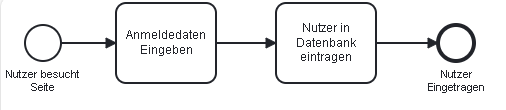
\includegraphics[width=15cm]{Figures/Beispiel2}
\decoRule
\caption[Prozess Block]{Erster Vollständiger Prozessblock}
\label{fig:Task}
\end{figure}

Events können allerdings auch während eines Prozesses auftreten. Wollen wir in unserem Beispiel einführen, dass die Startseite besucht werden kann, ohne, dass direkt auf die Nutzer anlegen Seite weitergeleitet wird, so können wir eine neue Aufgabe und ein fangendes Event einführen. Abbildung 2.3 zeigt diesen Prozess. Er startet, indem ein Nutzer die von uns erstellte Website besucht. Im nächsten Schritt wartet das catching Event, bis der Nutzer sich dazu entscheidet einen neuen Account anzulegen. In Folge dessen verhält sich der Prozess so, wie im Beispiel aus Abbildung 2.2. Events welche während dem Prozess auftreten werden "Intermediate Events" genannt.

\begin{figure}
\centering
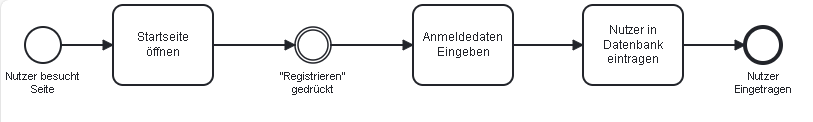
\includegraphics[width=15cm]{Figures/Beispiel3}
\decoRule
\caption[Intermediate Events]{Beispiel für ein intermediate Event}
\label{fig:Task}
\end{figure}

\subsection{Mögliche Verzweigungen}
 
In nun folgenden Abschnitt wollen wir uns mit Möglichkeiten beschäftigen den Sequenzfluss zu verzweigen. Hierzu bieten BPMN einige sogenannte „Gateways.“ Um Gateways darzustellen, werden Rauten verwendet. Unterschiedliche Gateways haben unterschiedliche Symbole in den Rauten eingezeichnet. Sie sind dafür da, den Verlauf des Prozesses aufzuteilen und wieder korrekt zusammenzufügen. Wenn ein Gateway den Verlauf des Prozesses aufspaltet, so muss immer ein zweites Gateway den Verlauf wieder zusammenfügen. Eine Ausnahme hierfür wäre, wenn der Prozess in einer Verzweigung durch ein Endevent terminiert.
Um unser bislang erarbeitetes Beispiel etwas realitätsnaher zu gestalten, wollen wir eine neue Funktion einführen. Offensichtlich soll unsere Seite mehr Funktionen anbieten als neue Nutzer anzulegen. Die nächste logische Erweiterung ist eine Möglichkeit für bereits bestehende Kunden sich mit ihren vorhandenen Anmeldedaten einzuloggen. Hier spielt die erste Verzweigungsmöglichkeit eine Rolle. Da ein Nutzer immer entweder ein bestehendes Konto besitzt oder ein neues erstellen möchte, wird in jedem Durchlauf des Prozesses nur eine dieser Aktionen durchgeführt. Hier kann ein XOR-Gateway genutzt werden. Es ist zu erkennen durch ein X in der Raute. Es bietet die Möglichkeit zwischen unterschiedlichen Pfaden zu wählen. Im Beispiel aus Abbildung 2.4 sehen wir eine mögliche Verwendung für dieses Gateway. Nachdem der Nutzer auf der Startseite den entsprechenden Button betätigt, wird er entweder zur Anmeldung oder zur Registrierung weitergeleitet. In beiden Fällen muss er seine Daten angeben. Im Anschluss werden die zwei Äste wieder zusammengeführt und der Nutzer wird mit seinem zugehörigen Account auf der Seite angemeldet. Beim Zusammenführen der Äste, wartet das Gateway auf genau einen Token und gibt diesen dann weiter an das nächste Objekt. In diesem Beispiel ist der erste Flow-Block zu erkennen. Wird der Verlauf des Prozess durch ein XOR-Gateway aufgespalten und wieder zusammengeführt, so bilden alle Elemente innerhalb dieser Verzweigung im sogenannen "Exclisive-choice-Block." Abbildung 2.4 zeigt außerdem eine Mögliche Variante des XOR-Gateways. Wenn der Nutzer einen vorhandenen Account anmelden möchte, aber inkorrekte Anmeldedaten eingibt, so wird er auf die Startseite zurückgeleitet. Das XOR-Gateway kann also auch für Loops verwendet werden. Denselben Verlauf sehen wir, falls der Nutzer bei der Registrierung invalide Daten angeben möchte. Auch hier wird der Nutzer auf die Startseite zurückgeleitet. Hier ist zu erkennen, dass das zusammenführende Gateway durchaus auch vor dem aufspaltenden Gateway liegen kann. Es ist zusätzlich möglich auch mehr als nur zwei Mögliche Ausgänge an das Gateway anzubinden. 



\begin{figure}
\centering
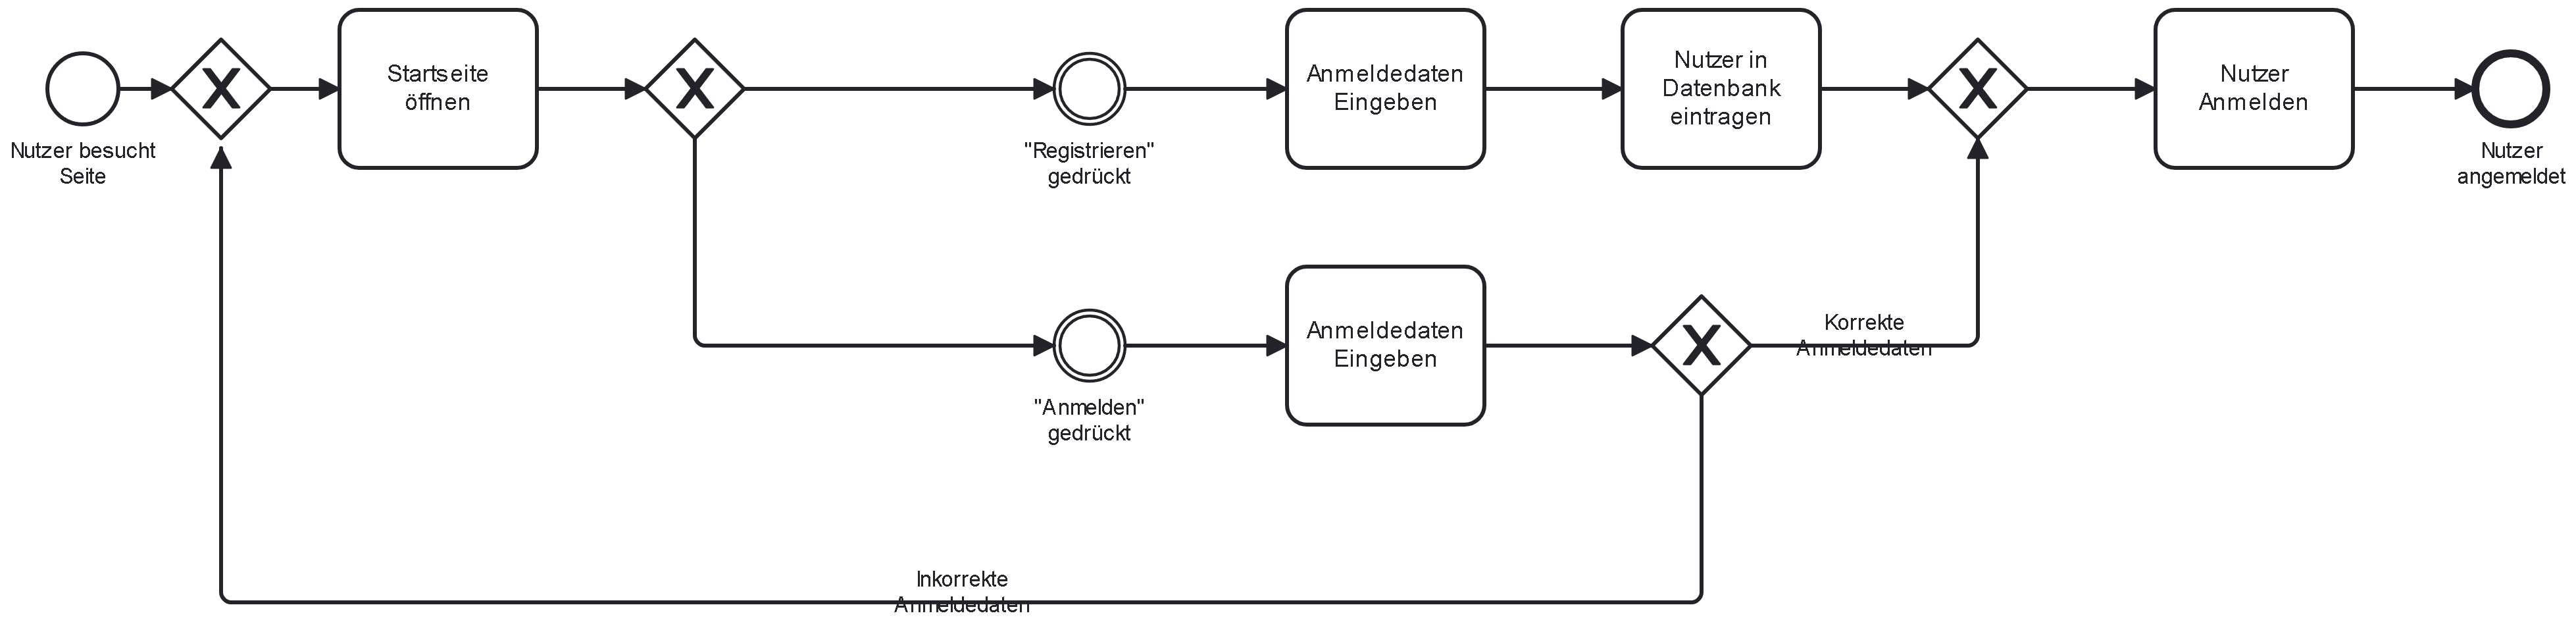
\includegraphics[width=15cm]{Figures/Beispiel5}
\decoRule
\caption[XOR-Gateway]{Exclusive Entscheidung - Das XOR-Gateway}
\label{fig:Task}
\end{figure}


Wir wollen nun ein weiteres Feature in unser Diagramm einfügen. Nachdem ein neuer Account erstellt wurde, soll dieser Nutzer nach wie vor angemeldet und auf die Homepage weitergeleitet werden. Zusätzlich soll er gleichzeitig auch für den Newsletter der Website eingetragen werden. Hierzu können wir ein weiteres Gateway nutzen. Das parallele Gateway wird in Abbildung 2.5 das erste Mal gezeigt. Es wird ebenfalls durch eine Raute dargestellt. Diese enthält allerdings ein + in ihrem Inneren. An diesem Gateway wird der Verlauf des Prozesses wieder aufgespalten. Anstelle von nur einem Strang werden hier aber alle Gelichzeitig ausgeführt. Das zusammenführende Gateway muss desshalb nicht blind den ersten Token weiterschicken, den es erhält, sondern wartet bis an allen Eingängen ein Token vorliegt, fügt diese wieder zusammen und gibt dann den Token weiter an das nächste Objekt. Hier können Schwierigkeiten auftreten, falls ein paralleler Zweig in einem Endevent endet. Bei der Modellierung eines Diagrammes muss dies also verhindert werden. 
\begin{figure}
\centering
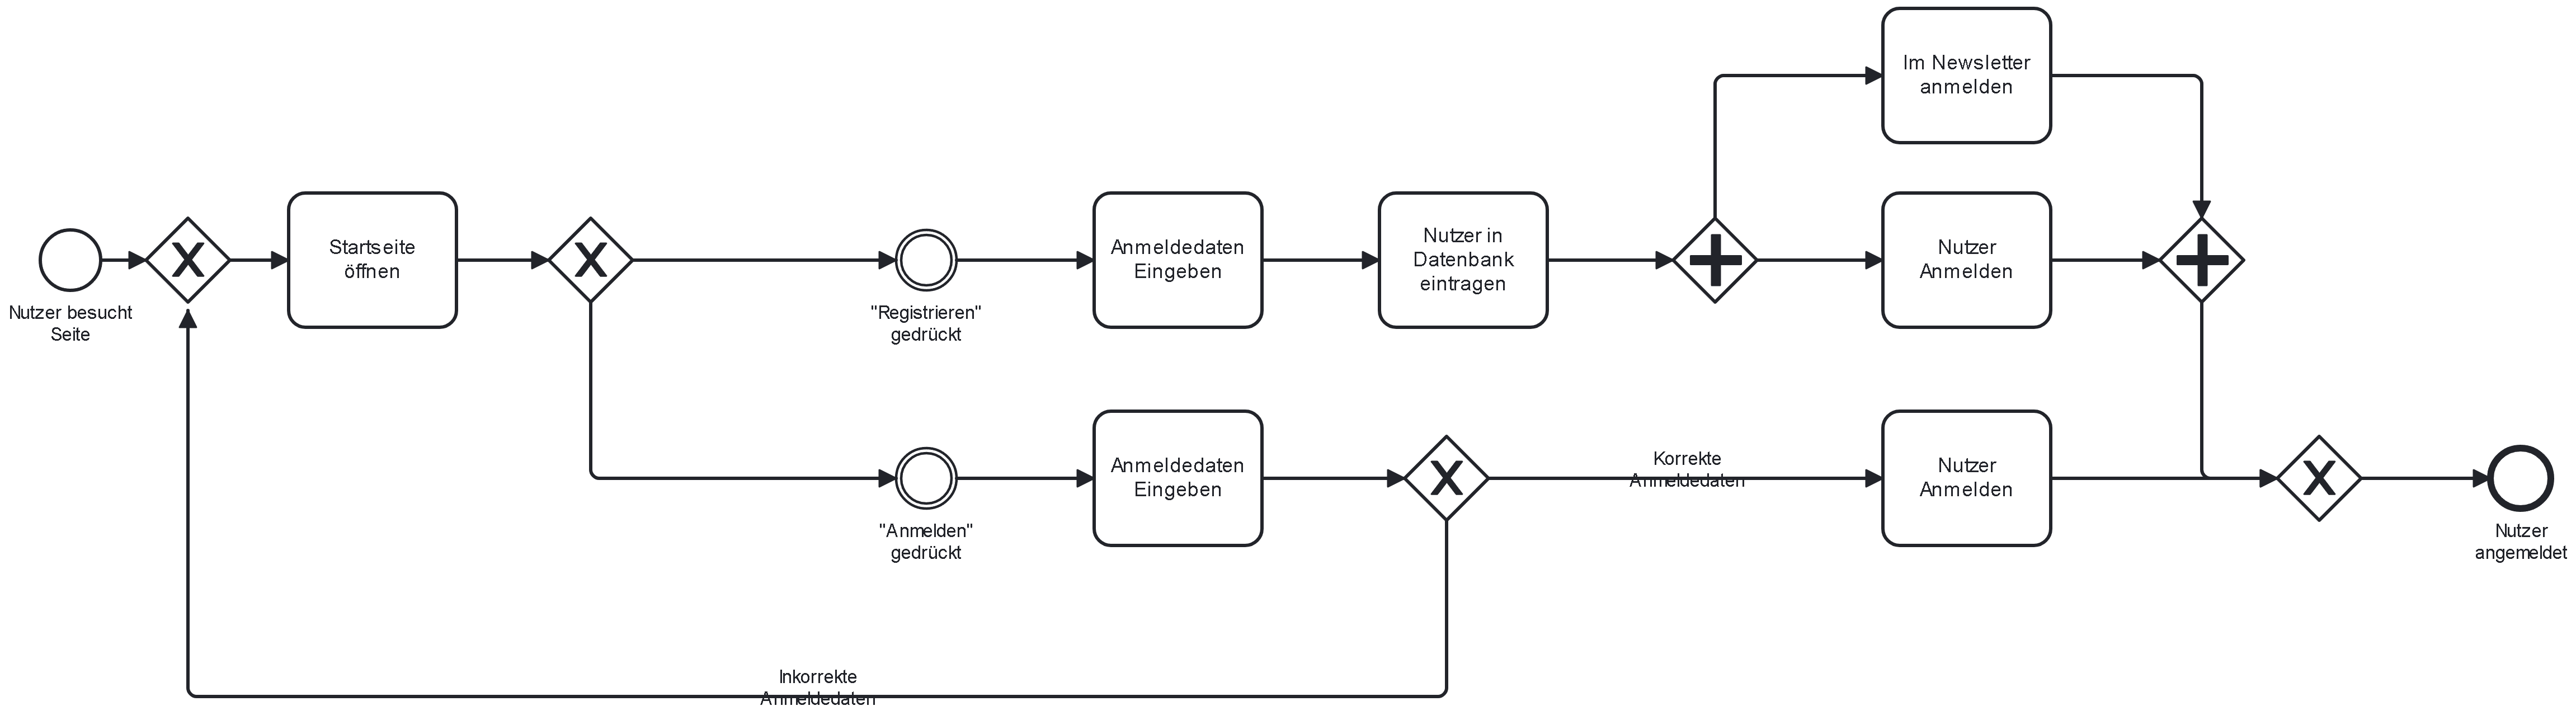
\includegraphics[width=15cm]{Figures/Beispiel6}
\decoRule
\caption[Paralell-Gateway]{Parallele Ausführung - Das Paralell-Gateway}
\label{fig:Task}
\end{figure}







